\documentclass[hidelinks]{article}
\usepackage[a4paper, total={7in, 10in}]{geometry}
\usepackage[dvipsnames]{xcolor}
\usepackage{amsmath}
\usepackage{tikz}
\usepackage{tkz-euclide}
\usepackage[unicode]{hyperref}
\usepackage[all]{hypcap}
\usepackage{fancyhdr}
\usepackage{amsfonts}
\usepackage[utf8]{inputenc}
\DeclareUnicodeCharacter{2212}{-}
\usepackage{amsmath}
\usepackage{array}
\usepackage{graphicx}
\mathchardef\mhyphen="2D % Define a "math hyphen"
\newcommand\rnumber{\mathop{r\mhyphen number}}
\graphicspath{ {./images/} }
\usetikzlibrary{angles,calc, decorations.pathreplacing}

\definecolor{carminered}{rgb}{1.0, 0.0, 0.22}
\definecolor{capri}{rgb}{0.0, 0.75, 1.0}
\definecolor{brightlavender}{rgb}{0.75, 0.58, 0.89}
\title{\textbf{MATH 61A Problem Set 1}}
\author{Allan Zhang}
\date{January 11, 2025}
\begin{document}
\hypersetup{bookmarksnumbered=true,}
\definecolor{darkspringgreen}{rgb}{0.09, 0.45, 0.27}
\definecolor{darkseagreen}{rgb}{0.56, 0.74, 0.56}
\definecolor{green(munsell)}{rgb}{0.0, 0.66, 0.47}
\pagecolor{white}
\color{black}
\maketitle

\section*{Question 1}
There is a simple identity where $\begin{pmatrix}n \\ k \end{pmatrix} = \begin{pmatrix}n \\ n-k \end{pmatrix}$ for any integer $n$ and any integer $k$ between 0 and $n$
\vspace{0.2cm}

(a) Explain why this is true in terms of the formula we derived for the binomial coefficients ($n$ choose $k$)

\[
    \begin{pmatrix}n \\ k \end{pmatrix} = \frac{n!}{k!(n-k)!} 
\]
\[
    \begin{pmatrix}n \\ n-k \end{pmatrix} = \frac{n!}{(n-k)!(n-(n-k))!} =  \frac{n!}{(n-k)!(n-(n-k))!} = \frac{n!}{(n-k)!k!} 
\]
As you can see, plugging the values into the formula we derived for the binomial coefficients provides us with the same expression after simplifying. Thus, $\begin{pmatrix}n \\ k \end{pmatrix} \text{ must equal } \begin{pmatrix}n \\ n-k \end{pmatrix}$
\vspace{0.2cm}

(b) Explain why this is true in terms of counting subsets.

Let's take a look at an example $\begin{pmatrix} 5 \\ 2\end{pmatrix}$ 

If we have the set $\{1, 2, 3, 4, 5\}$, the subets we can create are 
\[
    \{1, 2\}, \{1, 3\}, \{1, 4\}, \{1, 5\}, \{2, 3\}, \{2, 4\}, \{2, 5\}, \{3, 4\}, \{3, 5\}, \{4, 5\}
\]
There are 10 unique subsets in this sitatuion. Now, let us consider $\begin{pmatrix} 5\\ 3 \end{pmatrix}$, which is $\begin{pmatrix} n \\ n-k \end{pmatrix}$

Using the same set, the subsets we create are 
\[
    \{1, 2, 3\}, \{1, 2, 4\}, \{1, 2, 5\}, \{1, 3, 4\}, \{1, 3, 5\}, \{1, 4, 5\}, \{2, 3, 4\}, \{2, 3, 5\}, \{2, 4, 5\}, \{3, 4, 5\}
\]
This also provides us with 10 unique subsets. This isn't just a coincidence, as each subset in this case can be joined with another one of the subsets in the first case to create the whole set. Essentially, the subsets in the first case are the complements of the subsets in the second case. This is why $\begin{pmatrix}n \\ k \end{pmatrix} = \begin{pmatrix}n \\ n-k \end{pmatrix}$. Choosing a $k$ elements of a set is the same as choosing $n - k$ elements to exlude from the set.
\newpage
\section*{Question 2}
Prove the following fact by induction: for any natural number $n$, 
\[
    \sum_{i=0}^{n} i^2 = \frac{n(n+1)(2n+1)}{6}
\]
First, let us show that this is the case for the base case, $n = 0$
\[
    \sum_{i=0}^{0} i^2 = 0 = \frac{0(0+1)(2(0)+1)}{6} = 0
\]
Now, let us assume that this is true for $n = k$. Let us try to show that this is true for $k+1$ 
\[ 
    \sum_{i=0}^{k+1} i^2  = \sum_{i=0}^{k} i^2 + (k+1)^2 = \frac{k(k+1)(2k+1)}{6} + (k+1)^2
\]
\[
    \sum_{i=0}^{k} i^2 + (k+1)^2  = (k+1)\left (\frac{k(2k+1)}{6} + (k+1)\right)
\]
\[
    \sum_{i=0}^{k} i^2 + (k+1)^2  = (k+1)\left (\frac{2k+k+6k+6}{6} \right)
\]
\[
    \sum_{i=0}^{k} i^2 + (k+1)^2  = (k+1)\left (\frac{2k^2+7k+6}{6} \right)
\]
\[
    \sum_{i=0}^{k} i^2 + (k+1)^2  = (k+1)\left (\frac{(2k+3)(k+2)}{6} \right)
\]
\[
    \sum_{i=0}^{k} i^2 + (k+1)^2  = (k+1)\left (\frac{(2(k+1) + 1)(k+1) + 1)}{6} \right)
\]
Since this is exactly what we expected when setting $n=k+1$, we can say that this is true for all natural numbers $n$
\newpage
\section*{Question 3}

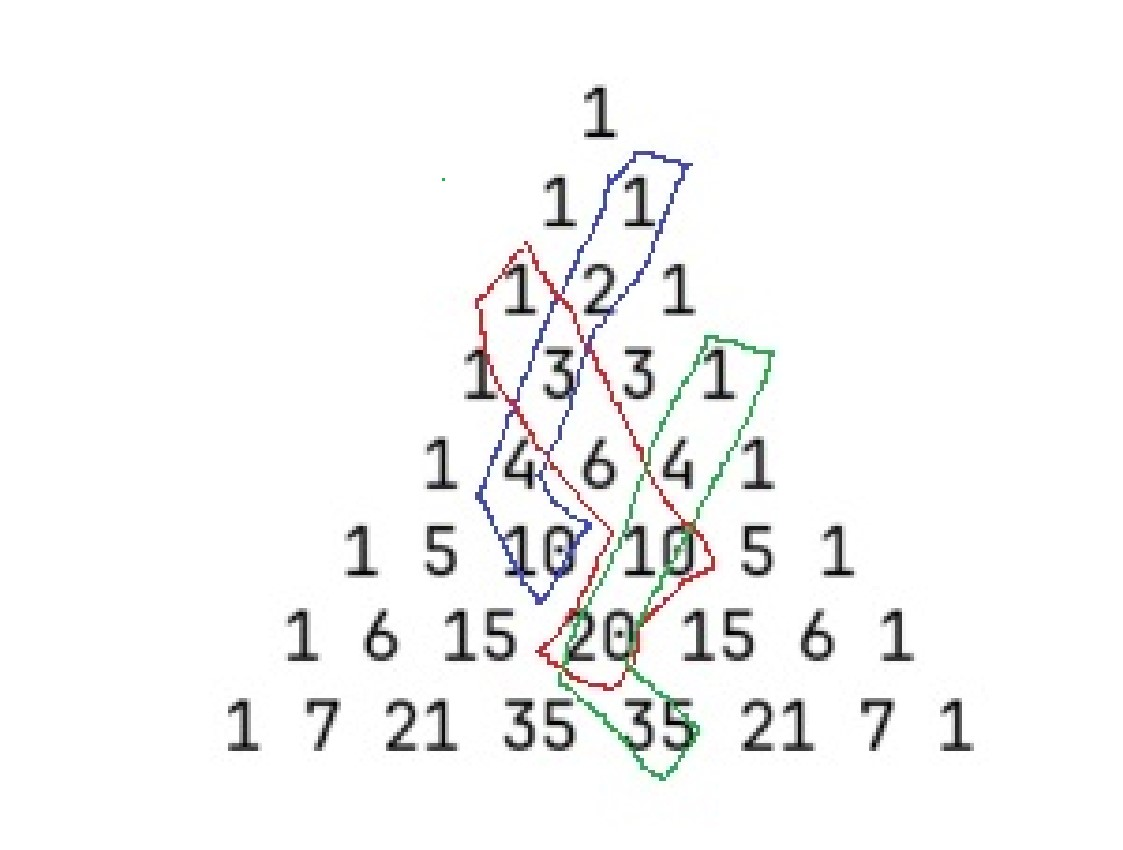
\includegraphics[scale=0.75]{pascal}

\end{document}

